\chapter{Generalization of Stair Climbing}

\section{Introduction}
Stair climbing is an important ADL. Exoskeletons need to be able to generate trajectories to climb the stairs. This work focuses on generating the trajectory from the start to the goal, not considering balance and stability. This research is not focused on the dynamics of maintaining upper body stability. It is directed on learning joint trajectories and therefore assumes that the goal point is within the exoskeletons support polygon using zero moment point \cite{kajita2003biped}.


By combining Stair Climbing LfD methods, step motions can be generalized and reproduced. Allowing for demonstrations of a single stair height to generate trajectories for different climbing heights simplifies the training process since all possible step heights cannot be collected for training data. Additionally, since the foot location is used as the training set, it abstracted the leg lengths and thus the person's height, allowing the motion to be reproduced for people of different heights. A similar recording method described in \cite{hicks2011lower} was used as the basis for the study. \autoref{fig:stairoverlay} shows the Vicon image of a person climbing the stairs. The collected data set was generalized with GMM and GMR. This collection and encoding method allowed robust data collection combined with a well-studied framework of teaching lower limb exoskeleton trajectories. Together, these methods allow a compilation of data to generalize a trajectory for stair climbing for people and stairs of different heights. This model shows that there is no need to retrain the trajectory for each person and different stair heights.



\begin{figure}
    \centering
    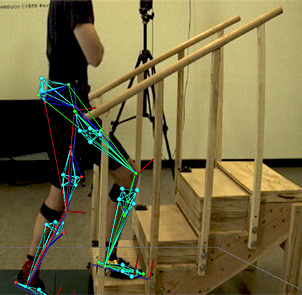
\includegraphics{images/stairs/mocap_overlay_stairs.jpg}
    \caption[Stair Mocap Overlay]{Subject with Mocap Overlay Climbing the Staircase. The stair case could be adjusted for the different trials by inserting wooden plates that were secured by bolts.}
    \label{fig:stairoverlay}
\end{figure}

\section{Learning of the Trajectories}
This work was published in IEEE Transactions on Medical Robotics and Bionics\cite{goldfarb2021towards}. \autoref{fig:stick} shows the coordinate layout used in this paper. The $X$ axis is perpendicular to the plane and is not considered since the exoskeleton does not have actuation along the $X$ axis. \autoref{fig:stick} shows a diagram of the subject in motion. In this diagram, the toe's position is controlled from the ground to the first step of the staircase. GMM (\autoref{eq:Mstep},\autoref{eq:Estep}) is used to learn the $Z$ and $Y$ marker position. The human demonstration (\autoref{chap:gaitdata}) was paired to find the stepping motion of the subject. Using GMR (\autoref{eq:GMR_Prop}, \autoref{eq:GMR_mu} ) the driving forcing is calculated. The forcing function is used to drive the model along the trajectory. DMPs (\autoref{eq:DMP_force}, \autoref{eq:DMP_Model} ) are used to replicate and alter the the trajectory to climb stairs of various heights.  


The limb length of the subject used for training was measured using a calibration phase. However, the limb length segments can be estimated using the height of the subject \cite{anthropomorphic}. It is assumed that the relative location of stairs is known with respect to the person. The motion has to be transferred to joint space using inverse kinematics of the leg. To avoid a collision of the toe with the lip of the stairs, a constraint that the foot must be parallel to the ground is imposed. In addition, some rehabilitation exoskeletons do not have actuated ankle joints and therefore cannot be controlled.  \autoref{eq:IK} is the inverse kinematics of the leg with a constrained ankle where hip: $q_1$, knee: $q_2$, ankle: $q_3$, thigh: $l_1$, shank: $l_2$, ankle height: $l_3$, foot length: $l_4$, $z_{toe}$ and $y_{toe}$ is the coordinate of the toe. Inverse kinematics allows for the encoding of the stair height instead of forward kinematics. 

\begin{equation} 
    \begin{aligned} 
        y' &= y_{toe} - l_4 \\ 
        z' &= z_{toe} + l_3 \\  
        \gamma &= y'^2 - z'^2 - l_1^2  - l_2^2 \\ 
        q_2 &= atan2 \Bigg( -\sqrt{1 - \frac{\gamma }{2 l_1^2 l_2^2}}, \frac{\gamma}{2 l_1^2 l_2^2}\Bigg)\\ 
        q_1 &= (atan2(z, y) - atan2( l_2 s_{q_2}, l_1 + l_2 c_{q_2})) + 0.5\pi \\ 
        q_3 &= (2\pi - q_1 - q_2) 
    \end{aligned} 
    \label{eq:IK} 
\end{equation} 

 
\begin{figure} 
    \centering 
    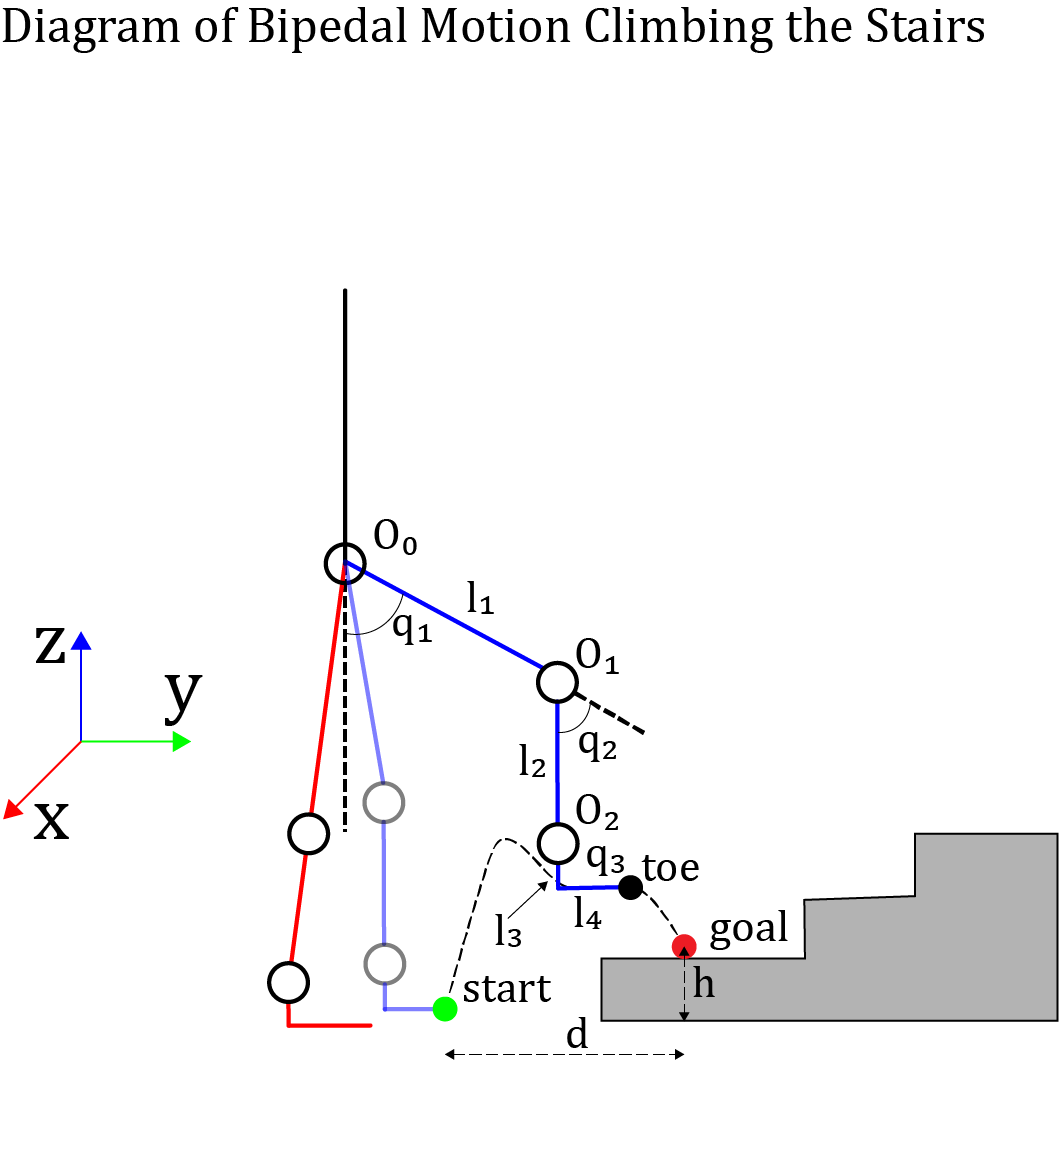
\includegraphics[scale=0.9]{images/stairs/stick.png}
    \caption[Stair Climbing Motion]{Figure representing the stair climbing motion of a 3 DoF leg. The start and goal are the parameters of the model shown as the distance $d$ and height $h$ from the toe to the stair. Each of the joint angles are calculated using inverse kinematics} 
    \label{fig:stick}
\end{figure} 

\autoref{fig:DTWStairs} shows the alignment of a trajectory against a demonstration. This demonstration was taken from stair climbing data set. The blue line is demo 1, and the orange line is demo 2. DTW aligns demo 2 with demo 1. The green line represents the aligned trajectory, and the red line represents a polynomial fit to the aligned trajectory. The cost map shows the closest fit of points from $P$ to $T$. The white spots are the hills, and the black spots are the valleys, with the path being the minimum cost from start to goal. The total path cost associated with the Euclidean was $17652.35$, and the cost of the Manhattan path was $33.50$. These are the costs of aligning the demonstration with the model trajectory. The Manhattan metric had a much lower cost than the Euclidean metric, allowing for a better fit. 

\begin{figure}[h]
     \centering 
     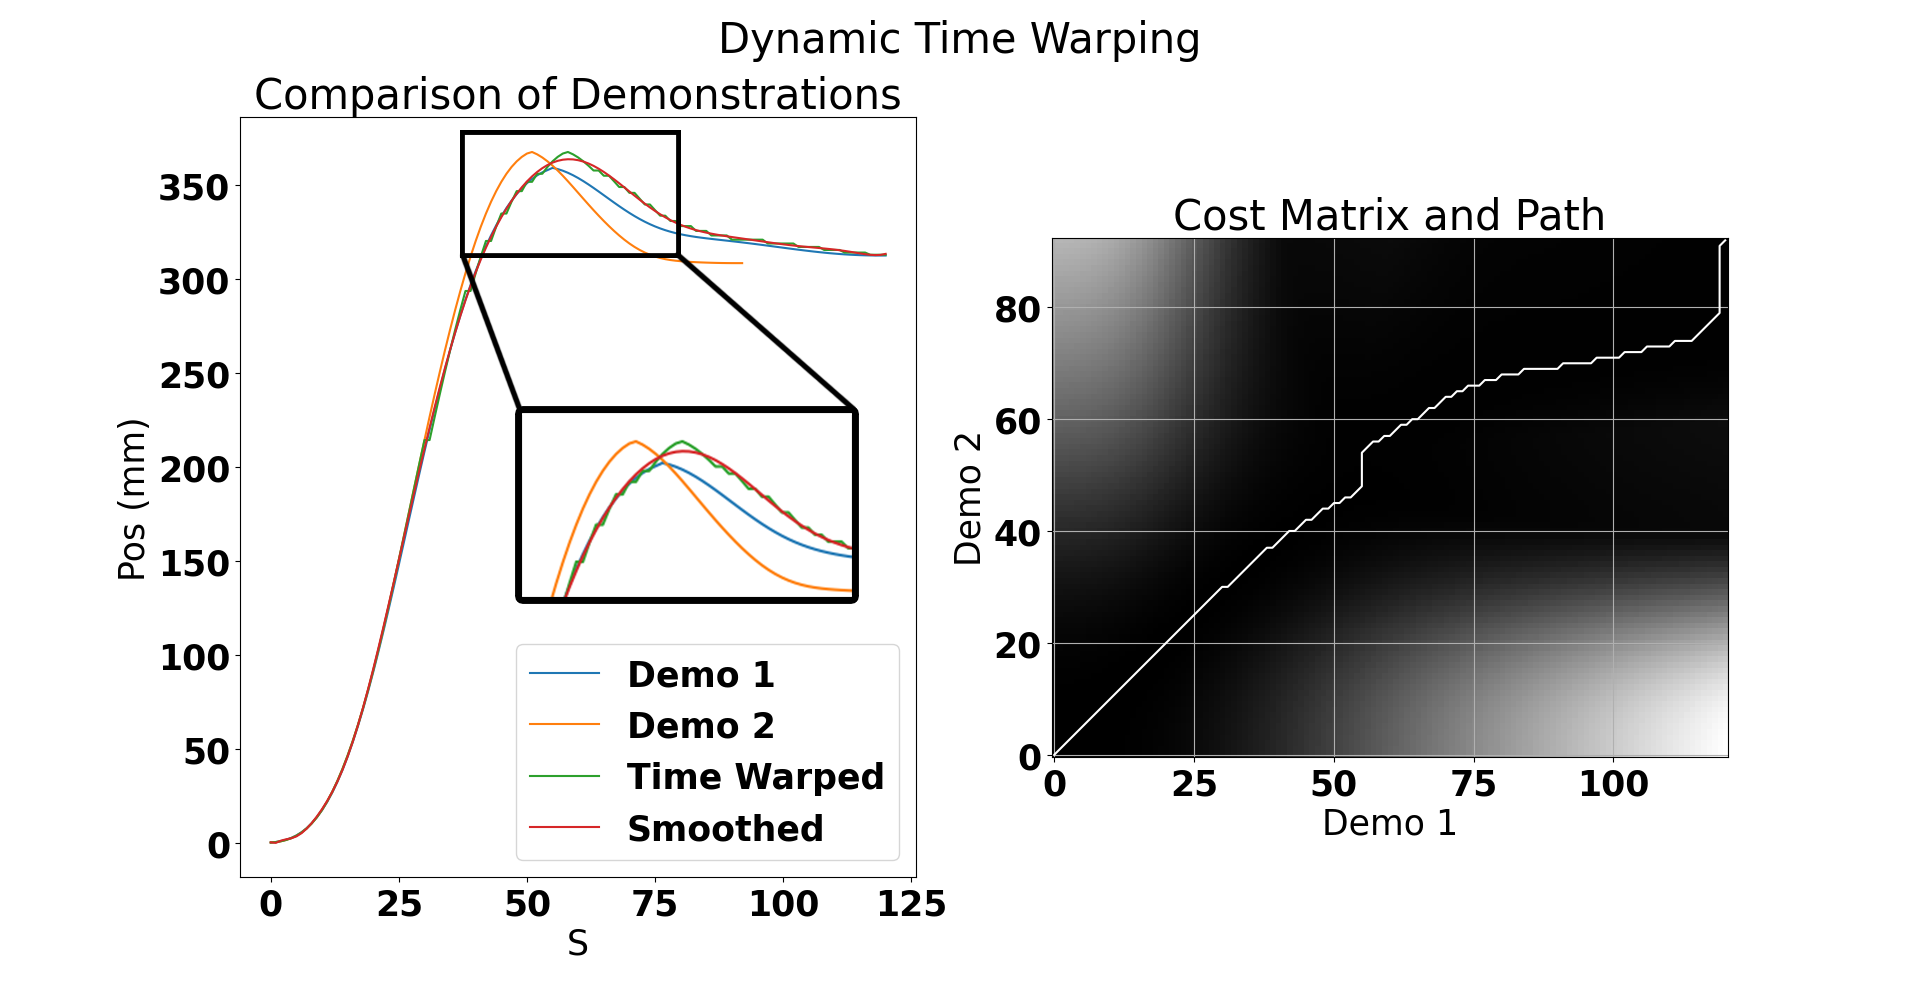
\includegraphics[width=\textwidth]{images/stairs/DTW_annotated.png} 
     \caption[Polynomial Smoothing of DTW]{Two demos being aligned using DTW and a smoothed trajectory. Blue line: demo 1. Orange line: demo 2. Green line: aligned trajectory. Red line: Polynomial smooth trajectory. The cost map shows the distance between the points.} 
     \label{fig:DTWStairs} 
\end{figure} 



The BIC score was used to optimize the number of required bins for the GMM process. \autoref{fig:BIC} shows the BIC score calculated for several bin sizes (1-25) for the $ Y $ and $ Z $ trajectories of the toe marker. This calculation limits the number of bins. The two graphs are generated using a single demonstration from each of the eight subjects in the config0 data set (see \autoref{tab:stairs}). The optimal number of bins for the $Z$ axis is 11 bins, and the optimal number of bins for the $Y$ axis is 14 bins. 


\begin{figure}[h!]
   \begin{subfigure}{\linewidth} 
    \centering 
    \ContinuedFloat
    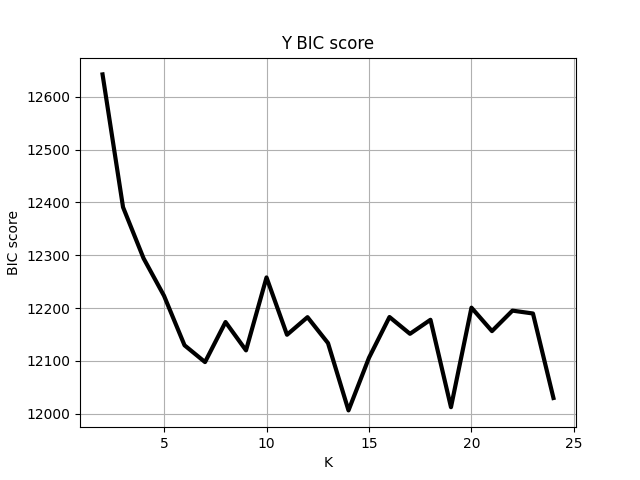
\includegraphics[ scale=0.6]{images/stairs/ybic7.png}
    \caption[BIC Score for $Y$ Toe]{BIC score for toe marker $Y$ position trajectory. The BIC score has its first local minimum at a size of 14 bins.} 
    \label{fig:BICY} 
  \end{subfigure}  
\begin{subfigure}{\linewidth} 
    \centering 
    \ContinuedFloat
    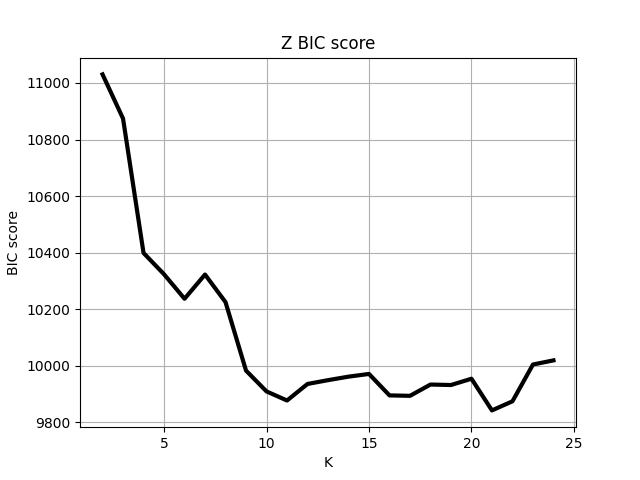
\includegraphics[ scale=0.6]{images/stairs/zbic6.png} 
    \caption[BIC Score for $Z$ Toe]{BIC score for toe marker $Z$ position trajectory. The BIC score has its first local minimum at a size of 11 bins.} 
    \label{fig:BICZ} 
  \end{subfigure}  
    \caption[Stair BIC Score]{The BIC score (smaller is better) was calculated for numerous bins size for the $Y$ and $Z$ trajectory.} 
    \label{fig:BIC} 
\end{figure}  

To find the number of subjects required to train the model. The demonstration trajectories were randomly sampled to avoid bias. The number of samples used to train the model was varied from 1 to 7 training demonstrations. Several demonstrations were excluded due to obstructed marker data. \autoref{tab:error} shows the imitation cost for a model trained with a single subject and a model trained using multiple subjects (see \autoref{eq:metric}). Both models were compared against a demonstration that was not used to train either model; this demonstrated that increasing the number of demonstrations reduces the metric of imitation and can follow the desired trajectories closer.   


\begin{table}[h]
\large 
     \centering 
     \begin{tabular}{||c|| c c ||}  
     \hline 
         Axis     & Y & Z  \\ [0.5ex]  
         \hline\hline 
         Single subject   & 138.01 & 67.86  \\  
         \hline 
         Multiple subjects & 70.7 & 25.63  \\ 
         \hline      
     \end{tabular} 
     \caption[Stair Imitation Cost]{Imitation cost (smaller is better) comparing models trained on a single subject to that trained on multiple subjects.  } 
     \label{tab:error} 
\end{table} 

\autoref{fig:trajLearning} shows the result of the learning of the $Y$ and $Z$ models using config0 subject data(see \autoref{tab:stairs}). The thick lines represent the generated model learned from the demonstrations using the optimal number of bins and demonstrations. The oscillations are caused by the DTW fitting of the demonstrations and the polynomial smoothing. The demonstrations with few points are being fit to the models with more points. The polynomial fitting ensures that the trajectories are smooth and not jagged.

\begin{figure}[h!] 
  \centering 
  \begin{subfigure}{\linewidth} 
    \centering 
    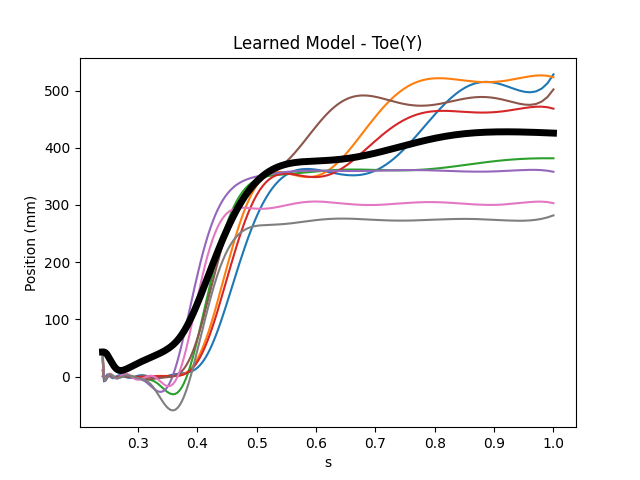
\includegraphics[ scale=0.6]{images/stairs/ylearn7.png} 
    \caption[$Y$ Marker Position Trajectory]{Comparison of learning the $Y$ marker position trajectory} 
    \label{fig:compY} 
  \end{subfigure} 
  \begin{subfigure}{\linewidth}
    \centering 
    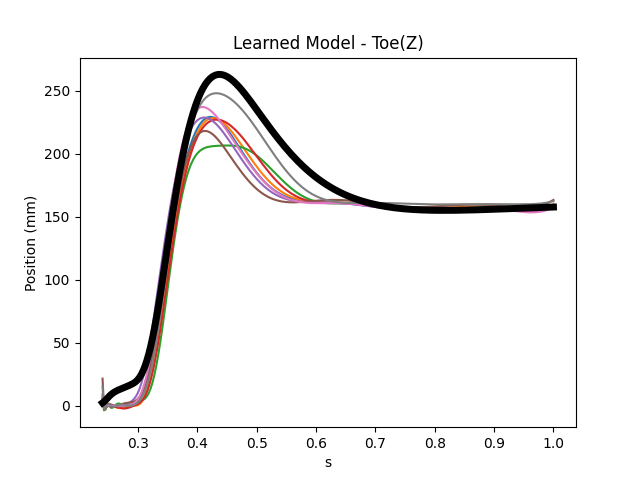
\includegraphics[ scale=0.6]{images/stairs/zlearn6.png} 
    \caption[$Z$ Marker Position Trajectory]{Comparison of learning the $Z$ marker position trajectory} 
    \label{fig:compZ} 
  \end{subfigure}   
  \caption[Stair Imitation model]{Imitation model for the toe position for climbing a stair. The $Z$ position is height of the toe relative to the floor and the $Y$ position is where the toe lands relative to the body. The thick line is the imitation model. The models used the optimized number of bins calculated from the BIC score.} 
  \label{fig:trajLearning} 
  
\end{figure}   




\section{Application of Generalized Stair Climbing}


\autoref{fig:singleSubject} shows a comparison of the model reproducing the motion of climbing several different stair heights. The solid line is the raw trajectory, and the dotted line is the reproduced line. The model's height was changed using DMPs by altering the goal ($g$). Each solid line represents the marker trajectories, and the dotted lines represent the reproduced trajectories. The model was compared against a demonstration that was not used for the model's training. The model was able to follow a foot trajectory for different stair heights. The trajectory of the different stair heights was not one of the demonstrations used to train the model.

\begin{figure}[h]
    \centering
    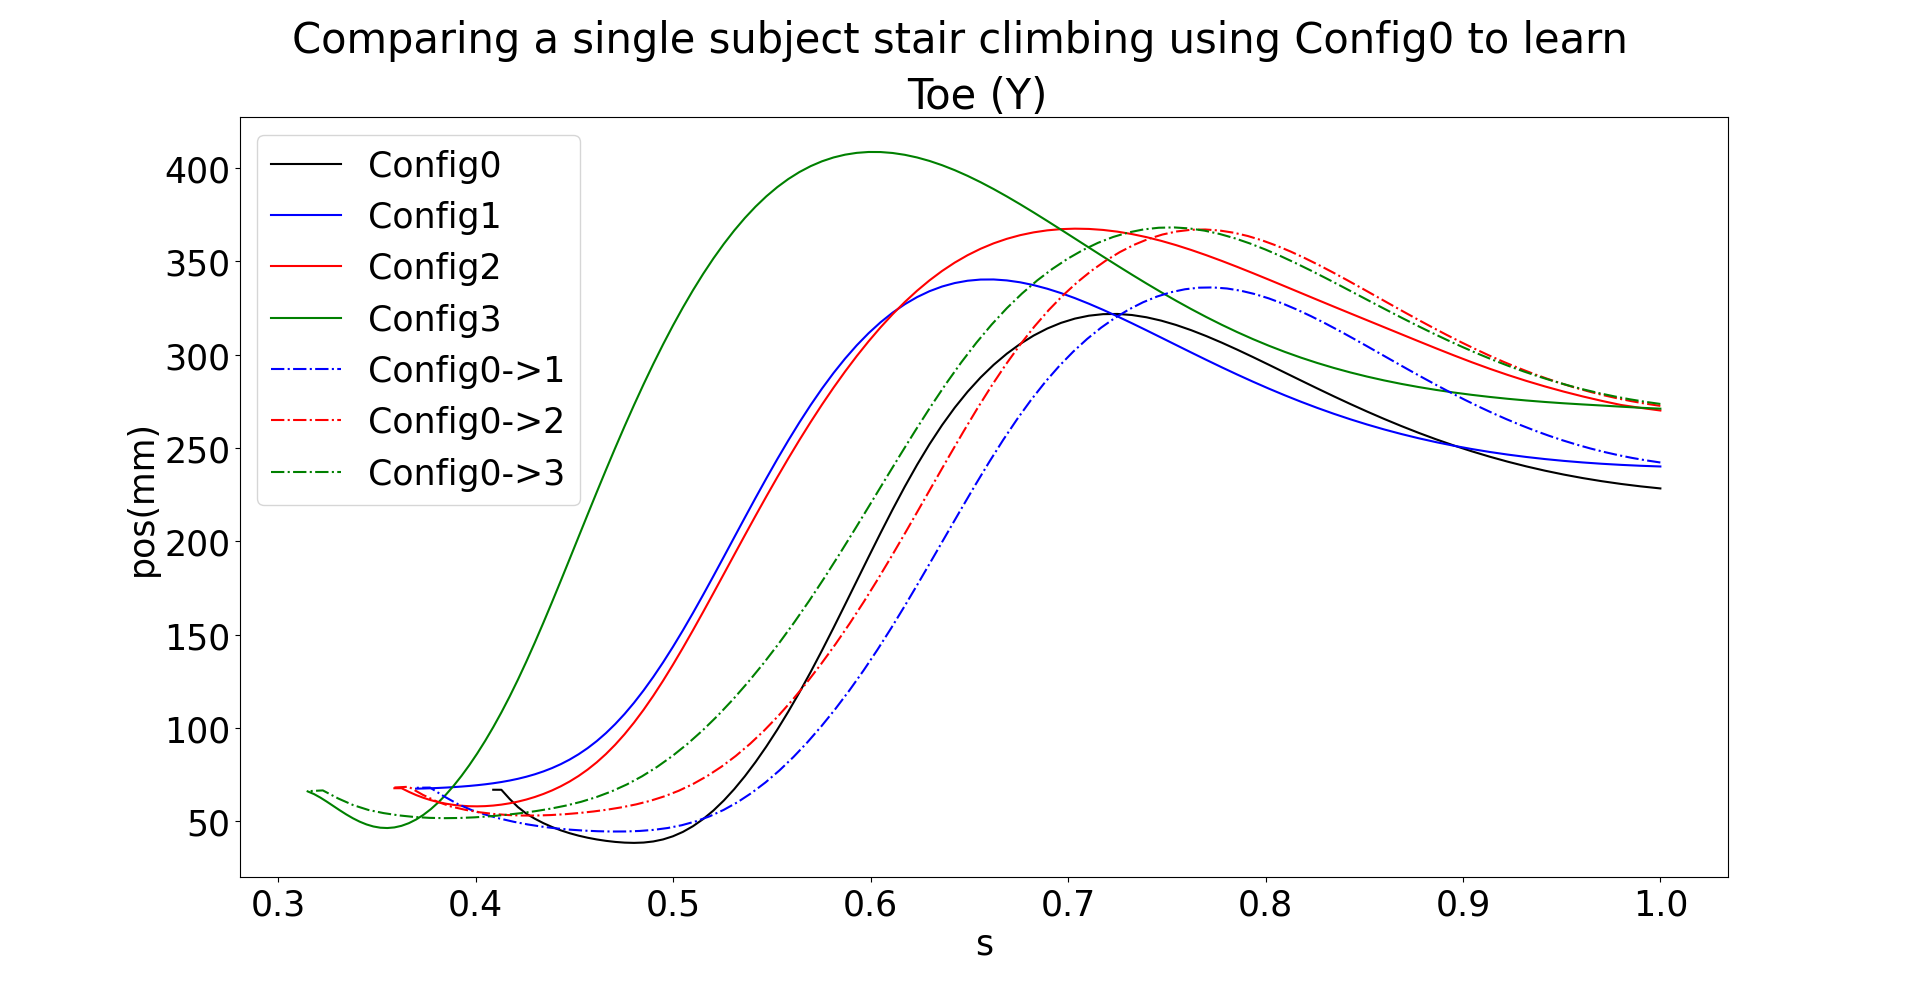
\includegraphics[scale=0.3]{images/stairs/compareHeihgts.png}
    \caption[Reproducing the Motion Climbing Different]{A model trained on single subject and single configuration, reproducing the motion climbing different stair heights. The solid lines are the marker trajectories. The dotted lines are the reproduced trajectories using the model}
    \label{fig:singleSubject}
\end{figure}

The inverse kinematics and the anthropomorphic parameters were used to calculate the desired joint angle for the exoskeleton. \autoref{fig:stairsclimbing} shows the movement of the leg through a stepping trajectory. Here the location of the toe is being controlled by controlling the joint angles. In this model, the ankle is constrained to be parallel to the ground. This constraint is to prevent the toe from catching on the edge of the stairs.


\begin{figure}[h!]
  \centering 
  \begin{subfigure}{\linewidth} 
    \centering
    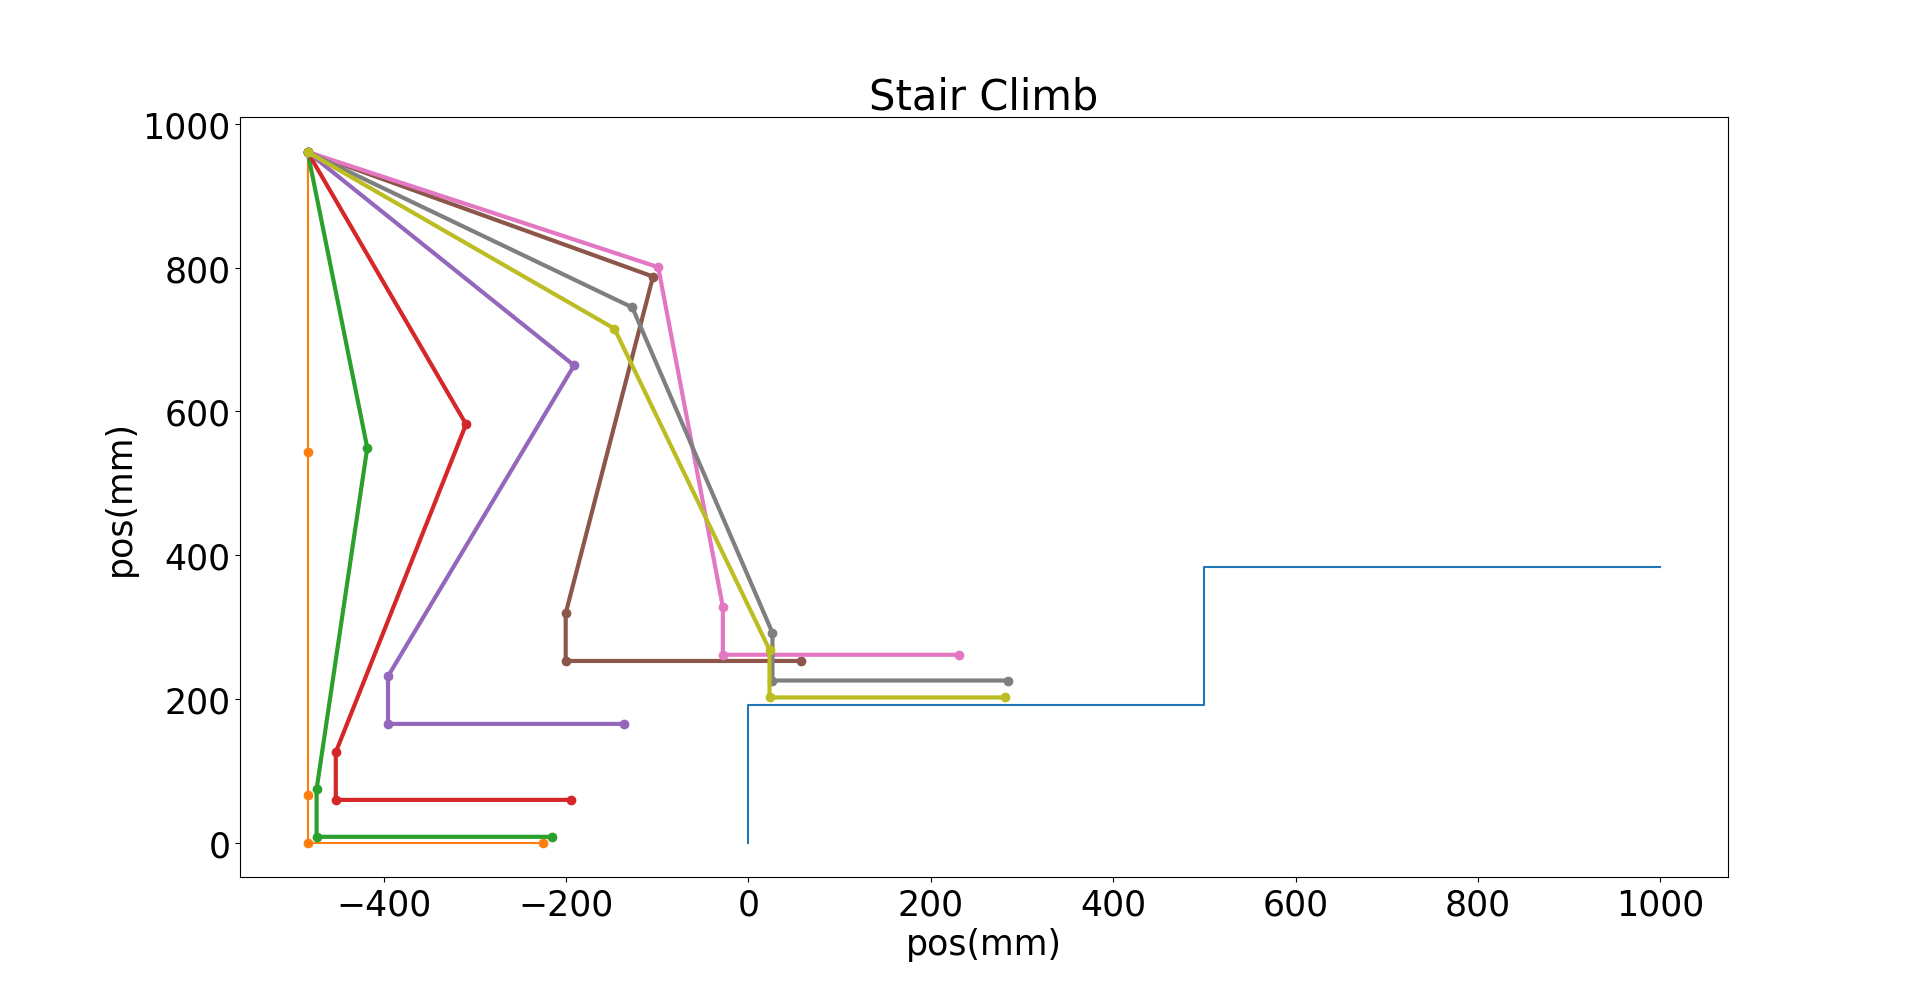
\includegraphics[scale=0.3]{images/stairs/stairs_climb.png}
    \caption[Stepping Trajectory]{The leg motion over the stepping trajectory while keeping the ankle parallel with the ground. Inverse kinematics was then used to solve for the joint angles.}
    \label{fig:stairsclimbing}
  \end{subfigure} 
    \begin{subfigure}{\linewidth} 
    \centering 
    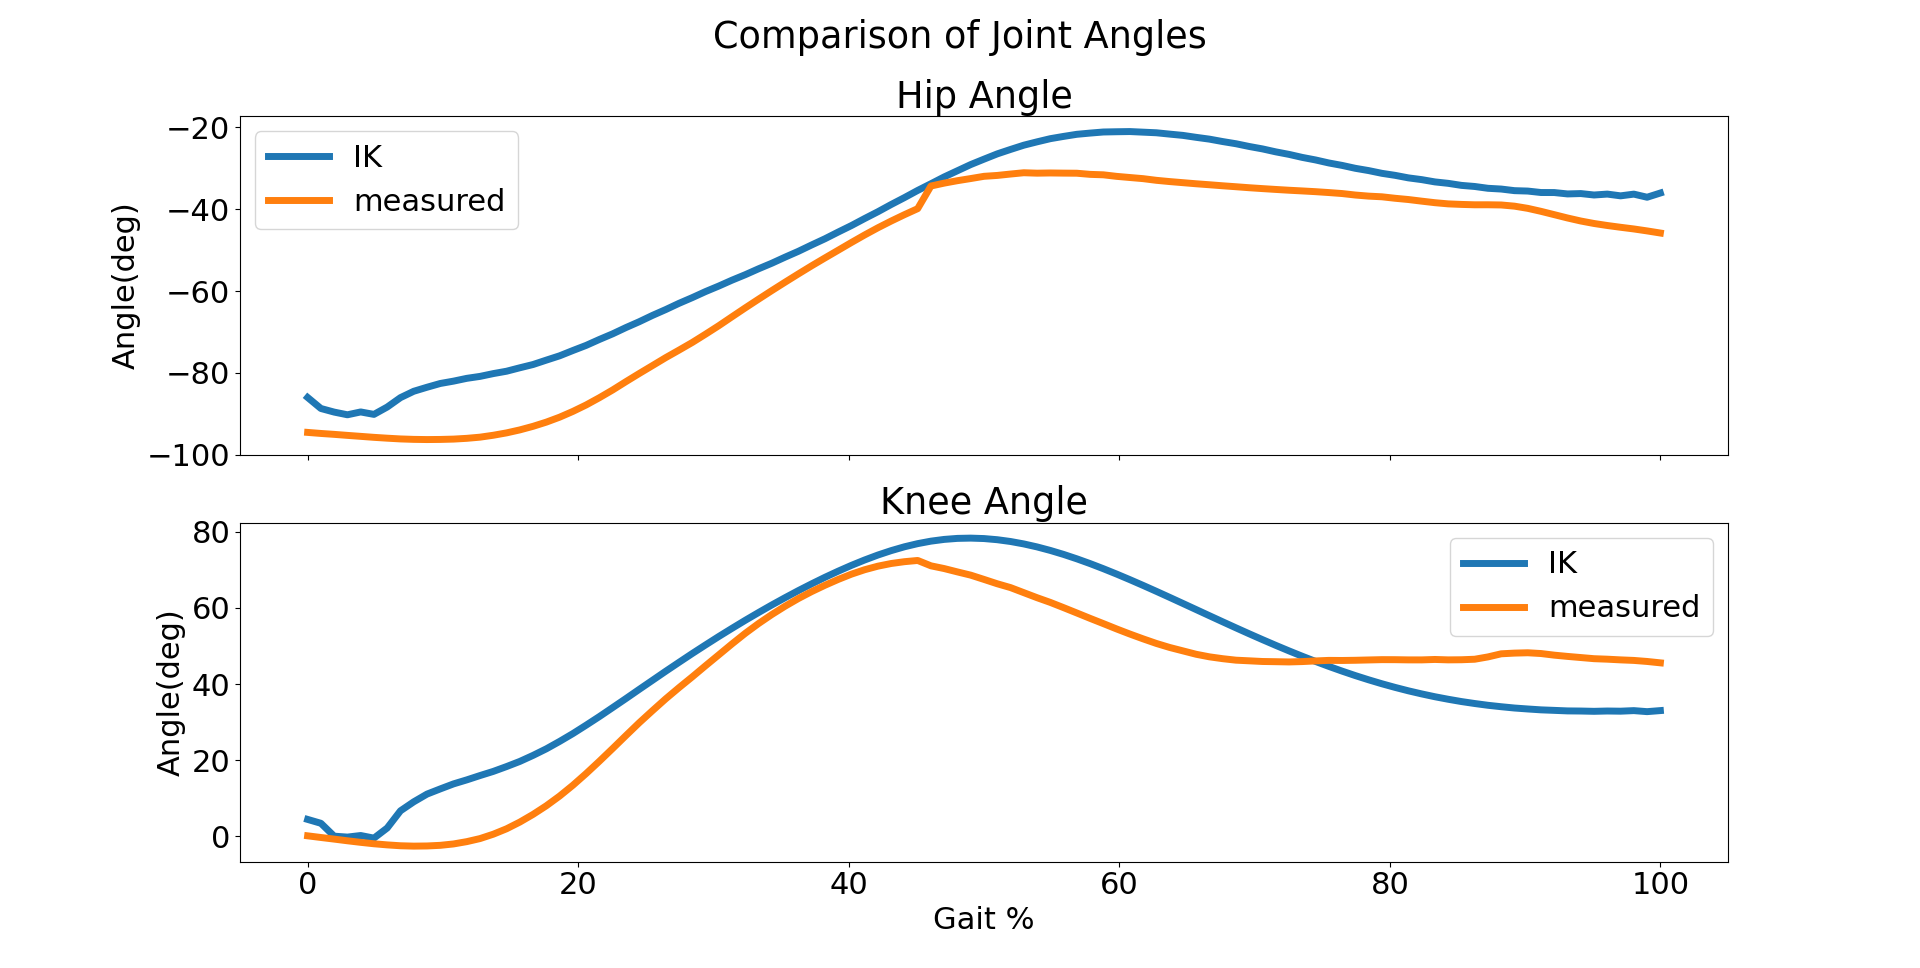
\includegraphics[ scale=0.3]{images/stairs/joint_angle_stairs_no_ankle.png} 
    \caption[Stair IK Path]{Comparison of the joint angle. The IK path was calculated using the inverse kinematics and the toe tip. The measured joint angle are independently measured using the Vicon tracking software.}  
    \label{fig:config3} 
  \end{subfigure}   
  \caption[Stair Control]{Control of the leg from the ground to the first step. The joint angle are calculated and compared to the measured joint angles. } 
  \label{fig:singleSubject} 
\end{figure}   


\section{Contributions}

This contribution of this method was to show how to build an imitation model by learning stair climbing trajectories using mocap and GMM/GMR. This work showed a trajectory generation of the joint trajectories for the exoskeletons joint angles to be generalized so it can be used by people of all leg lengths on variable stair heights. This method allows the model to handle different stair heights by changing the start and goal inputs to the DMP controller. Unlike other methods that rely on hand-generated trajectory generation from start to the goal, this method allows biological stair climbing trajectories to be used that can be dynamically manipulated to climb different stair heights.


% The stair location can be found using LIDAR or distance sensors (see \autoref{fig:sensors}). 